\documentclass{article}
\usepackage[english]{babel}
\usepackage[utf8]{inputenc}
\usepackage{amsmath,amssymb}
\usepackage{parskip}
\usepackage{graphicx}
\usepackage{dsfont}
\usepackage{dsfont}
\usepackage{relsize}
\usepackage{array}
\newcommand{\bigsigma}{\makebox{\Huge\ensuremath{\sigma}}}
\newcommand{\bigpi}{\makebox{\Huge\ensuremath{\Pi}}}
\newcolumntype{C}[1]{>{\centering\let\newline\\\arraybackslash\hspace{0pt}}m{#1}}
\usepackage[top=2.5cm, left=3cm, right=3cm, bottom=4.0cm]{geometry}
\usepackage[table]{xcolor}
\usepackage[utf8]{inputenc}
\usepackage{textcomp}
\usepackage[utf8]{inputenc}
\usepackage{amsmath}
\usepackage{amssymb}
\usepackage{xcolor}
\usepackage{listings}
\usepackage{xstring}
\usepackage{graphicx}
\usepackage[export]{adjustbox}
\usepackage{setspace}

\definecolor{dkgreen}{rgb}{0,0.6,0}
\definecolor{ltgray}{rgb}{0.5,0.5,0.5}

\makeatletter
\newif\ifcolname
\colnamefalse

\def\keywordcheck{%
\IfStrEq*{\the\lst@token}{select}{\global\colnametrue}{}%
\IfStrEq*{\the\lst@token}{where}{\global\colnametrue}{}%
\IfStrEq*{\the\lst@token}{from}{\global\colnamefalse}{}%
\color{blue}%
}
\def\setidcolor{%
\ifcolname\color{purple}\else\color{black}\fi%
}
\makeatother

\lstset{%
    backgroundcolor=\color{white},
    basicstyle=\footnotesize,
    breakatwhitespace=false,
    breaklines=true,
    captionpos=b,
    commentstyle=\color{dkgreen},
    deletekeywords={...},
    escapeinside={\%*}{*)},
    extendedchars=true,
    frame=single,
    keepspaces=true,
    language=SQL,
    otherkeywords={is},
    morekeywords={*,modify,MODIFY,...},
    keywordstyle=\keywordcheck,
    identifierstyle=\setidcolor,
    numbers=left,
    numbersep=15pt,
    numberstyle=\tiny,
    rulecolor=\color{ltgray},
    showspaces=false,
    showstringspaces=false, 
    showtabs=false,
    stepnumber=1,
    tabsize=4,
    title=\lstname
}

\newcommand{\tablespace}{\\[1.25mm]}
\newcommand\Tstrut{\rule{0pt}{2.6ex}}         % = `top' strut
\newcommand\tstrut{\rule{0pt}{2.0ex}}         % = `top' strut
\newcommand\Bstrut{\rule[-0.9ex]{0pt}{0pt}}   % = `bottom' strut
\title{Assignment-3 CS303}
\author{Shashank P \\ 200010048}
\date{\today}

\begin{document}
\maketitle




\section{Problem 1}
Design a database for an automobile company to provide to its dealers to assist them in maintaining
customer records and dealer inventory and to assist sales staff in ordering cars.
Each vehicle is identified by a vehicle identification number ( VIN ). Each individual vehicle is a
particular model of a particular brand offered by the company (e.g., the XF is a model of the car brand
Jaguar of Tata Motors). Each model can be offered with a variety of options, but an individual car may
have only some (or none) of the available options. The database needs to store information about models,
brands, and options, as well as information about individual dealers, customers, and cars. Your design
should include an E-R diagram, a set of relational schemas, and a list of constraints, including
primary-key and foreign-key constraints.


\begin{figure}[!ht]
  \begin{center}
    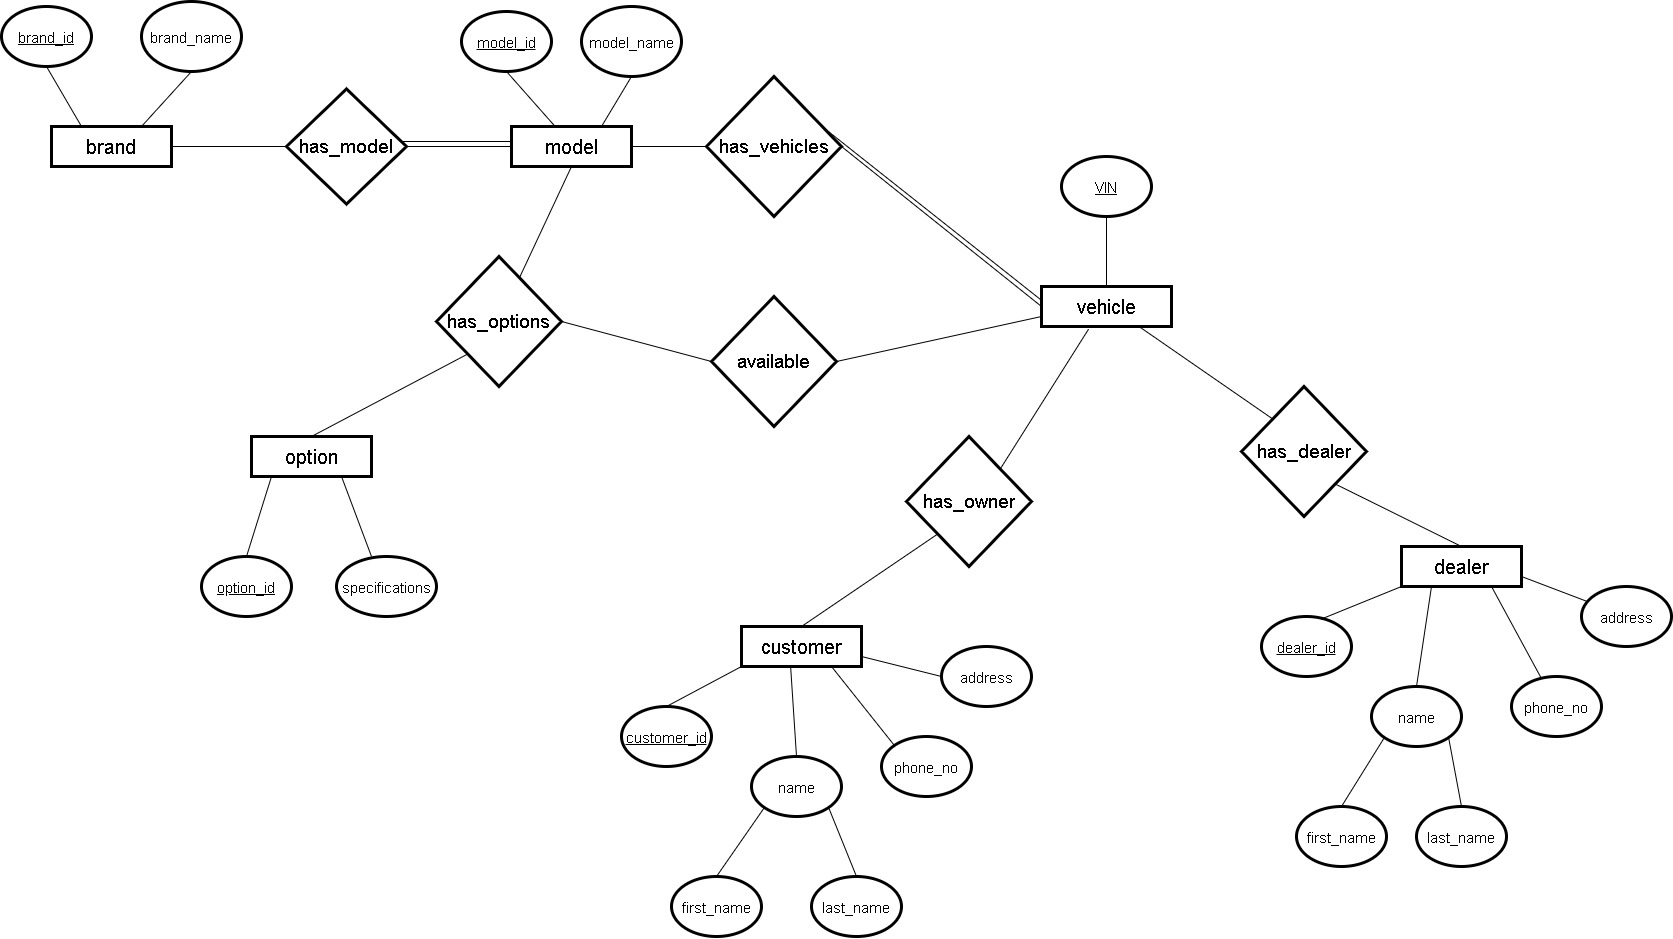
\includegraphics[scale=0.3]{1.jpg}
  \caption{ER Model}
  \end{center}
\end{figure}

\subsection{Schema}
\onehalfspacing
\begin{center}
  brand (\underline{brand\_id}, brand\_name), \\
  model (\underline{model\_id}, mdoel\_name), \\
  option (\underline{option\_id}, specifications), \\
  vehicle (\underline{VIN}), \\
  customer (\underline{customer\_id}, name, phone\_no, address), \\
  dealer (\underline{dealer\_id}, name, phone\_no, address), \\
  has\_model (\underline{brand\_id} ref. \textbf{brand}, \underline{model\_id} ref. \textbf{model}), \\
  has\_options (\underline{model\_id} ref. \textbf{model}, \underline{option\_id} ref. \textbf{option}), \\
  has\_vehicles (\underline{model\_id} ref. \textbf{model}, \underline{VIN} ref. \textbf{vehicle}), \\
  available ((\underline{model\_id}, \underline{option\_id}) ref. \textbf{has\_options}, \underline{VIN} ref. \textbf{vehicle}), \\
  has\_owner (\underline{VIN} ref. \textbf{vehicle}, \underline{customer\_id} ref. \textbf{customer}), \\
  has\_dealer (\underline{VIN} ref. \textbf{vehicle}, \underline{dealer\_id} ref. \textbf{dealer}) \\
\end{center}

\section{Problem }
Design a database for a world-wide package delivery company (e.g., DHL or Fed EX ). The database
must be able to keep track of customers (who ship items) and customers (who receive items); some
customers may do both. Each package must be identifiable and trackable, so the database must be able to
store the location of the package and its history of locations.
Locations include trucks, planes, airports, and warehouses. Your design should include an E-R diagram, a
set of relational schemas, and a list of constraints, including primary-key and foreign-key constraints.

\newpage
\begin{figure}[!ht]
  \begin{center}
    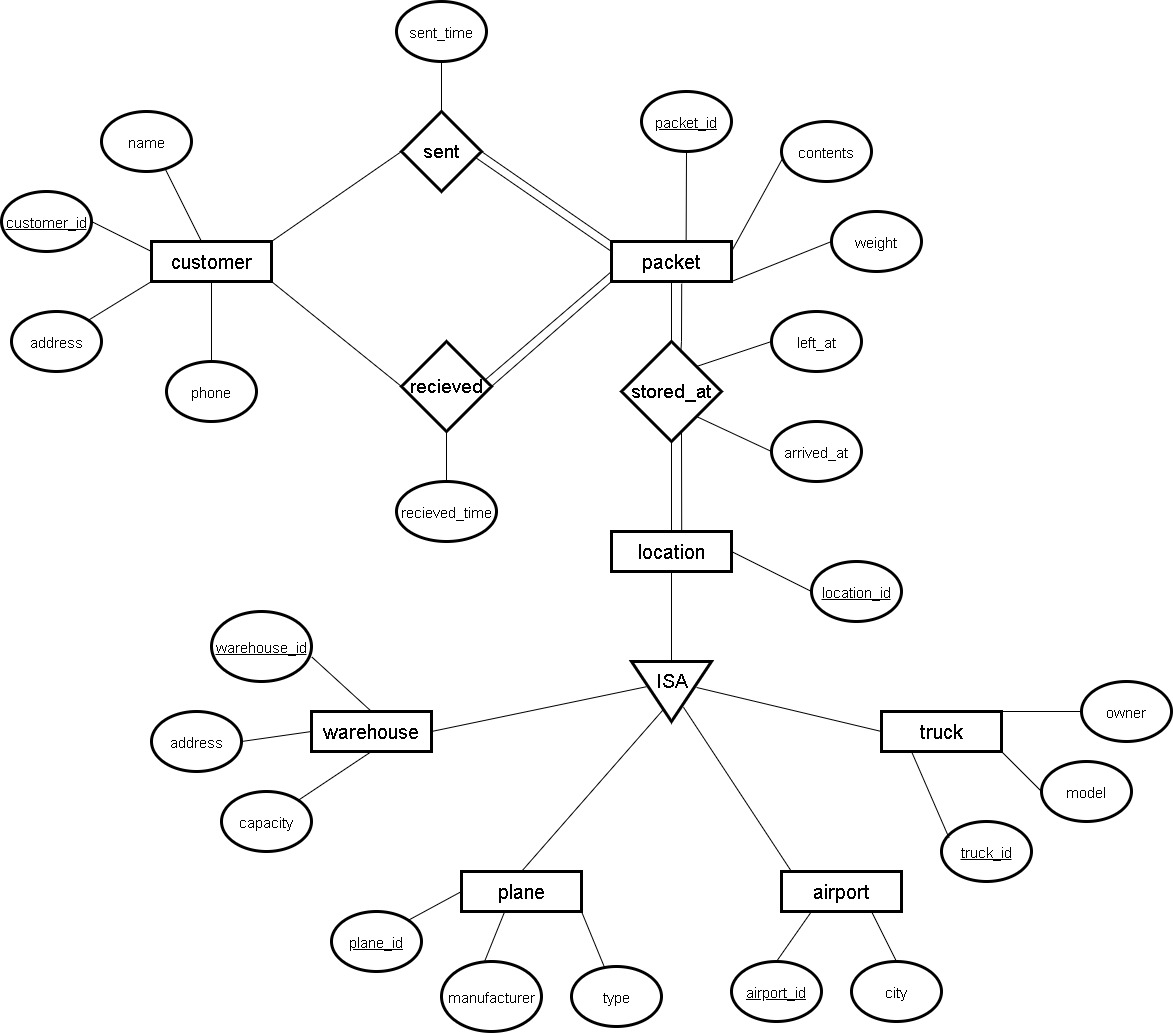
\includegraphics[scale=0.4]{2.jpg}
  \caption{ER Model}
  \end{center}
\end{figure}

\newpage
\subsection{Schema}
\onehalfspacing
\begin{center}
  customer (\underline{customer\_id}, name, phone, address), \\
  packet (\underline{packet\_id}, contacts, weight), \\
  location (\underline{location\_id}), \\
  warehouse (\underline{warehouse\_id} ref. \textbf{location(location\_id)}, address, capacity), \\
  plane (\underline{plane\_id} ref. \textbf{location(location\_id)}, manufacturer, type), \\
  airport (\underline{airport\_id} ref. \textbf{location(location\_id)}, city), \\
  truck (\underline{truck\_id} ref. \textbf{location(location\_id)}, model, owner), \\
  sent (\underline{customer\_id} ref. \textbf{customer}, \underline{packet\_id} ref. \textbf{packet}, sent\_time), \\
  recived (\underline{customer\_id} ref. \textbf{customer}, \underline{packet\_id} ref. \textbf{packet}, recieved\_time), \\
  stored\_at (\underline{packet\_id} ref. \textbf{packet}, \underline{location\_id} ref. \textbf{location}, arrived\_at, left\_at), \\
\end{center}


\end{document}
